\documentclass[tikz,landscape]{standalone}

\usepackage{geometry}
    \geometry{paperheight=78cm, paperwidth=110cm, lmargin=20mm, rmargin=20mm, tmargin=20mm, bmargin=20mm}

\usepackage{pgfplots}
    \pgfplotsset{compat=newest}
    \usetikzlibrary{arrows.meta}
    \usetikzlibrary{backgrounds}
    \usetikzlibrary{calc}
    \usetikzlibrary{positioning}
    \usetikzlibrary{patterns}
    \usetikzlibrary{fit}

\usepackage[T1]{fontenc}
\usepackage[largesc]{newtxtext}

\usepackage[scaled]{helvet}
\usepackage[T1]{fontenc}
    \renewcommand\familydefault{\sfdefault}

\usepackage{newtxmath}
\usepackage{siunitx}
\usepackage{tabularx}
\usepackage{booktabs}
\usepackage[version=4]{mhchem}
    \mhchemoptions{layout=stacked}
\usepackage{xcolor}
    \definecolor{TUMBlue}        {RGB/cmyk}{  0,101,189 / 1.  ,0.43,0.  ,0.  }
    \definecolor{TUMBlack}       {RGB/cmyk}{  0,  0,  0 / 0.  ,0.  ,0.  ,1.  }
    \definecolor{TUMBlueDarker}  {RGB/cmyk}{  0, 51, 89 / 1.  ,0.57,0.12,0.7 }
    \definecolor{TUMBlueLighter} {RGB/cmyk}{152,198,234 / 0.42,0.09,0.  ,0.  }
    \definecolor{TUMOrange}      {RGB}{227, 114, 34}
    \definecolor{TUMGreen}       {RGB}{162, 173, 0}
    \definecolor{tab10blue}{HTML}{1f77b4}
    \definecolor{tab10orange}{HTML}{ff7f0e}
    \definecolor{tab10green}{HTML}{2ca02c}  
    \definecolor{tab10red}{HTML}{d62728}
    \colorlet{pcolor}{tab10red}
    \colorlet{hcolor}{black}
    \colorlet{h2color}{TUMOrange}
    \colorlet{ohcolor}{TUMGreen}
    \colorlet{h2ocolor}{TUMBlue}


\newcommand{\rate}[2]{
    \Large
    \begin{tabular}{l}
        \bfseries #1 \\
        #2
    \end{tabular}
}
\newcommand{\sirange}[3]{\SI{#1}{}\,\text{--}\,\SI{#2}{#3}}
\newcommand{\h}[1]{\textcolor{TUMBlueLighter}{\textbf{#1}}}


% layers
\pgfdeclarelayer{H}     % declare background layer
\pgfdeclarelayer{H2}    % declare background layer
\pgfdeclarelayer{OH}    % declare background layer
\pgfdeclarelayer{H2O}   % declare background layer
\pgfdeclarelayer{loss}  % declare background layer
\pgfsetlayers{background,H2O,OH,H2,H,main,loss}  % set the order of the layers (main is the standard layer)

\begin{document}
\pagestyle{empty}


%
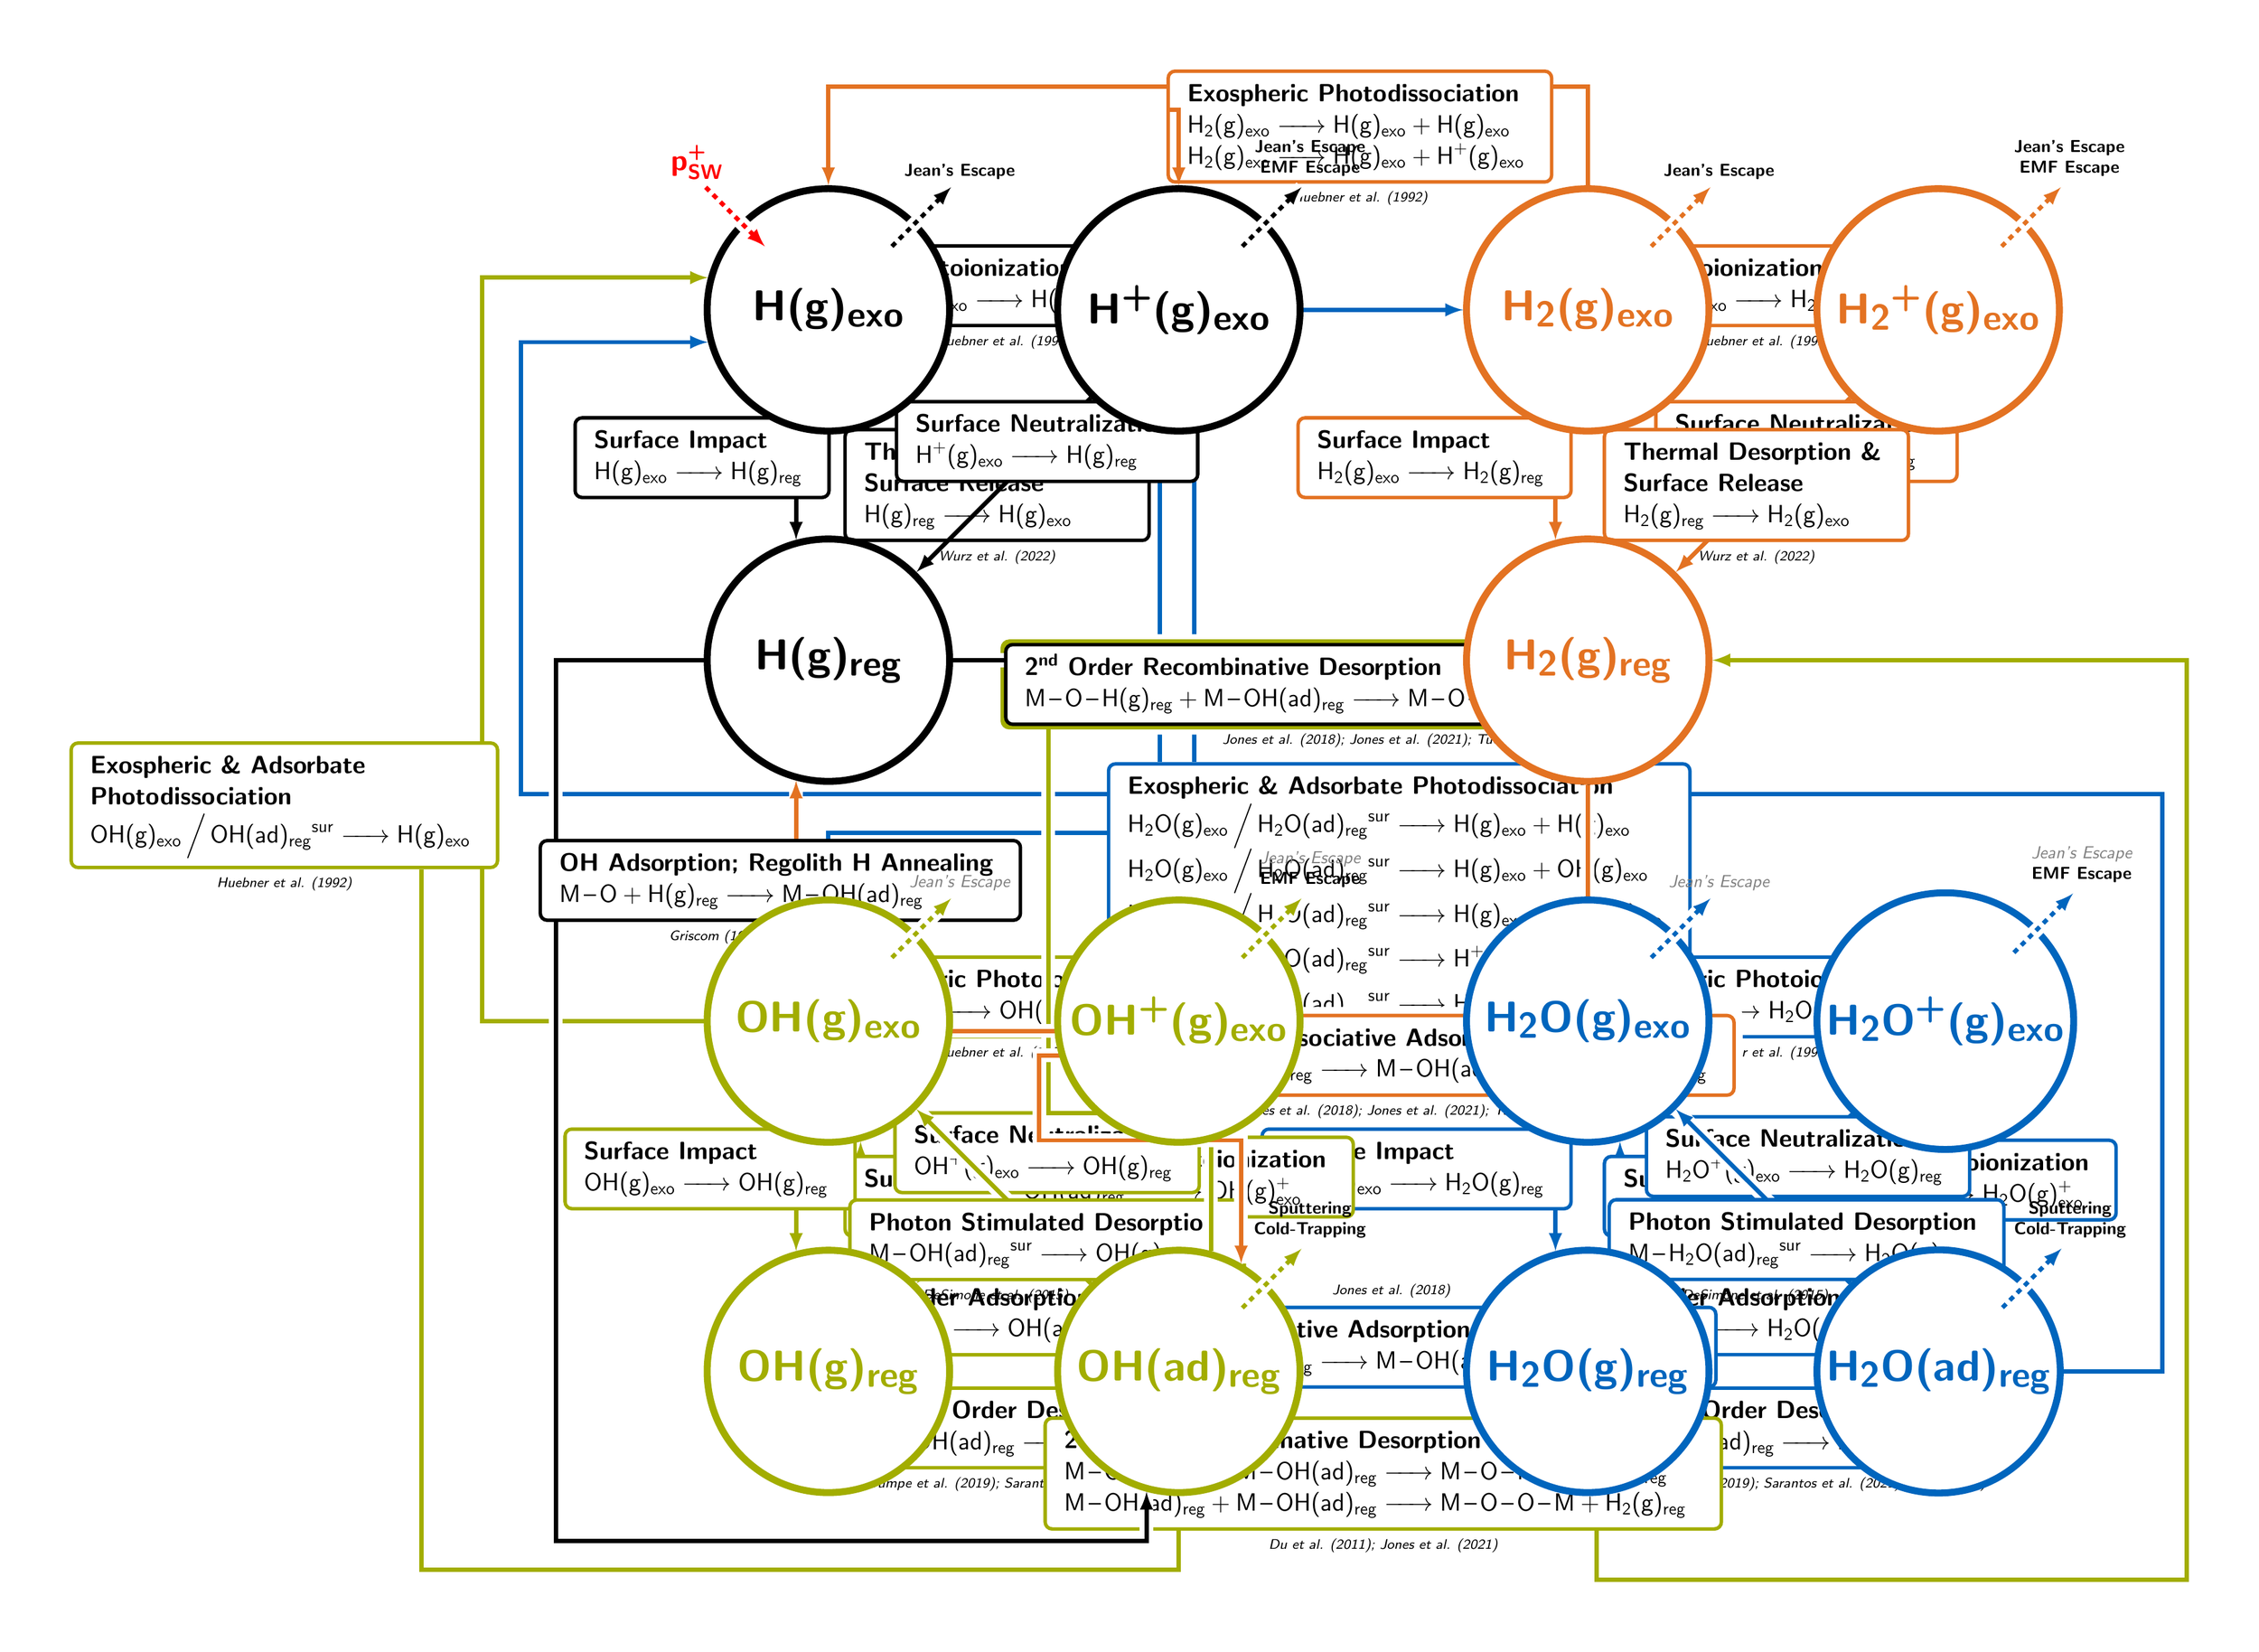
\begin{tikzpicture}[background rectangle/.style={fill=white},show background rectangle,inner frame sep=30px,
  sub/.style={circle,draw,line width=4pt,minimum size=140pt,anchor=mid,font={\bfseries\Huge},fill=white,align=center},
  path/.style={line width=2.5pt,-latex,font={\normalsize},},
  traj/.style={line width=2.5pt,-latex,font={\normalsize},},
  rate/.style={rounded corners,draw,solid,line width=2pt,fill=white,inner sep=5pt,font={\normalsize},text=black},
  every label/.style={draw=none,fill=none,font={\footnotesize\itshape},text=black},
  loss/.style={at end,above,xshift=5pt,text=black},
  source/.style={at end,above,xshift=-5pt,text=red,font={\bfseries\Huge},},
]
  % variables
  \def\innernodesep{.095\paperwidth}
  \def\outernodesep{.15\paperwidth}
  \def\whitelinewidth{8pt}

  % H nodes
  \node[hcolor,sub] (HGEXO) at (0,0) {\ce{H(g)_{exo}}};
  \node[hcolor,sub,right=\innernodesep of HGEXO] (HpGEXO) {\ce{H+(g)_{exo}}};
  \node[hcolor,sub,below=\innernodesep of HGEXO] (HGREG) {\ce{H(g)_{reg}}};


  % H2 nodes
  \node[h2color,sub,right=\outernodesep of HpGEXO] (H2GEXO) {\ce{H2(g)_{exo}}};
  \node[h2color,sub,right=\innernodesep of H2GEXO] (H2pGEXO) {\ce{H2+(g)_{exo}}};
  \node[h2color,sub,below=\innernodesep of H2GEXO] (H2GREG) {\ce{H2(g)_{reg}}};


  % OH nodes
  \node[ohcolor,sub,below=0.7*\outernodesep of HGREG] (OHGEXO) {\ce{OH(g)_{exo}}};
  \node[ohcolor,sub,right=\innernodesep of OHGEXO] (OHpGEXO) {\ce{OH+(g)_{exo}}};
  \node[ohcolor,sub,below=\innernodesep of OHGEXO] (OHGREG) {\ce{OH(g)_{reg}}};
  \node[ohcolor,sub,right=\innernodesep of OHGREG] (OHADREG) {\ce{OH(ad)_{reg}}};


  % H2O nodes  
  \node[h2ocolor,sub,right=\outernodesep of OHpGEXO] (H2OGEXO) {\ce{H2O(g)_{exo}}};
  \node[h2ocolor,sub,right=\innernodesep of H2OGEXO] (H2OpGEXO) {\ce{H2O+(g)_{exo}}};
  \node[h2ocolor,sub,below=\innernodesep of H2OGEXO] (H2OGREG) {\ce{H2O(g)_{reg}}};
  \node[h2ocolor,sub,right=\innernodesep of H2OGREG] (H2OADREG) {\ce{H2O(ad)_{reg}}};

  % switch to background layer
  \begin{pgfonlayer}{H}

  %%% rates
  %% H
  \draw[path,hcolor] (HGEXO.0) -- (HpGEXO.180) 
    node[rate,midway,above,yshift=-10pt,label={below:Huebner et al. (1992)}]{
      \rate{Photoionization}{\ce{H(g)_{exo} -> H(g)^+_{exo} }}
  };

  \draw[white,line width=\whitelinewidth] (HGREG.180) -- +(-3,0) |- ($(OHADREG.255)+(0,-1)$) -- (OHADREG.255);
  \draw[path,hcolor] (HGREG.180) -- +(-3,0) |- ($(OHADREG.255)+(0,-1)$) 
    node[rate,pos=0.125,right,xshift=-10pt,label={below:Griscom (1985); Jones et al. (2021)}]{
      \rate
        {\ce{OH} Adsorption; Regolith \ce{H} Annealing}
        {\ce{M-O + H(g)_{reg} -> M-OH(ad)_{reg}}}
  } -- (OHADREG.255);

  \draw[path,hcolor] (HGREG.75) -- (HGEXO.285)
    node[rate,midway,right,xshift=-10pt,label={below:Wurz et al. (2022)}]{
      \rate
        {Thermal Desorption \&\\\textbf{Surface Release}}
        {\ce{H(g)_{reg} -> H(g)_{exo}}}
  };

  \draw[traj,hcolor] (HGEXO.255) -- (HGREG.105) 
    node[rate,near start,left,xshift=20pt,]{
      \rate{Surface Impact}{\ce{H(g)_{exo} -> H(g)_{reg}}}
  };

  \draw[traj,hcolor] (HpGEXO.225) -- (HGREG.45) 
    node[rate,near start]{
      \rate{Surface Neutralization}{\ce{H^+(g)_{exo} -> H(g)_{reg}}}
  };

  \draw[white,line width=\whitelinewidth] (HGREG.0) -- (H2GREG.180);
  \draw[path,hcolor] (HGREG.0) -- (H2GREG.180)
    node[rate,pos=0.765,below,yshift=10pt,label={below:~~~~~~~~~~~~~~~~~~~~~~~~~~~~Jones et al. (2018); Jones et al. (2021); Tucker et al. (2018)}] (Htmp1) {
      \rate
        {2$^\text{nd}$ Order Recombinative Desorption}
        {\ce{M-O-H(g)_{reg} + M-OH(ad)_{reg} -> M-O-O-M + H2(g)_{reg}}}
  };

  \end{pgfonlayer}


  %% H2
  \begin{pgfonlayer}{H2}
  \draw[path,h2color] (H2GEXO.90) -- +(0,2) -| (HGEXO.90)
    node[rate,pos=0.15,below,yshift=10pt,label={below:Huebner et al. (1992)}] (H2tmp1) {
      \rate
        {Exospheric Photodissociation}
        {\ce{H2(g)_{exo} -> H(g)_{exo} + H(g)_{exo}}\\\ce{H2(g)_{exo} -> H(g)_{exo} + H^+(g)_{exo}}}
    };
  \draw[path,h2color] (H2tmp1.175) -| (HpGEXO.90); 

  \draw[path,h2color] (H2GEXO.0) -- (H2pGEXO.180) 
    node[rate,midway,above,yshift=-10pt,label={below:Huebner et al. (1992)}]{
      \rate
        {Photoionization}
        {\ce{H2(g)_{exo} -> H2(g)^+_{exo} }}
  };

  \draw[traj,h2color] (H2pGEXO.225) -- (H2GREG.45) 
    node[rate,near start]{
      \rate{Surface Neutralization}{\ce{H2^+(g)_{exo} -> H2(g)_{reg}}}
  };

  \draw[path,h2color] (H2GREG.75) -- (H2GEXO.285) 
    node[rate,midway,right,xshift=-10pt,label={below:Wurz et al. (2022)}]{
      \rate
        {Thermal Desorption \&\\\textbf{Surface Release}}
        {\ce{H2(g)_{reg} -> H2(g)_{exo}}}
  };

  \draw[traj,h2color] (H2GEXO.255) -- (H2GREG.105) 
    node[rate,near start,left,xshift=10pt,]{
      \rate{Surface Impact}{\ce{H2(g)_{exo} -> H2(g)_{reg}}}
  };

  \draw[white,line width=\whitelinewidth] (H2GREG.270) -- +(0,-5) -| (HGREG.255);
  \draw[path,h2color] (H2GREG.270) -- +(0,-5) -| (HGREG.255)
    node[rate,pos=0.10,below,yshift=10pt,label={below:Jones et al. (2018); Jones et al. (2021); Tucker et al. (2018)}] (H2tmp2) {
      \rate
        {2$^\text{nd}$ Order Dissociative Adsorption}
        {\ce{M-O + H2(g)_{reg} -> M-OH(ad)_{reg} + M-O + H(g)_{reg}}}
  };
  \draw[white,line width=\whitelinewidth] (H2tmp2.180) -- +(-1.7,0) |- ($(OHADREG.60)+(0,2.5)$) -- (OHADREG.60);
  \draw[path,h2color] (H2tmp2.180) -- +(-1.7,0) |- ($(OHADREG.60)+(0,2.5)$) -- (OHADREG.60);
  \end{pgfonlayer}


  %% OH
  \begin{pgfonlayer}{OH}
  \node (H2tmp3) [rate,white,inner sep=3pt,fit=(H2tmp2)] {};
  \node (Htmp3) [rate,white,inner sep=4pt,fit=(Htmp1)] {};

  \draw[path,ohcolor] (OHGREG.75) -- (OHGEXO.285) 
    node[rate,midway,right,xshift=-10pt,]{
      \rate{Surface Release}{\ce{OH(g)_{reg} -> OH(g)_{exo}}}
  };

  \draw[traj,ohcolor] (OHGEXO.255) -- (OHGREG.105) 
    node[rate,near start,left,xshift=35pt,]{
      \rate{Surface Impact}{\ce{OH(g)_{exo} -> OH(g)_{reg}}}
  };

  \draw[path,ohcolor] (OHGEXO.180) -| +(-4.5, 1) |- (HGEXO.165)
    node[rate,pos=0.12,left,xshift=10pt,label={below:Huebner et al. (1992)}] (OHtmpphoto) {
      \rate
        {Exospheric \& Adsorbate\\\textbf{Photodissociation}}
        {\ce{OH(g)_{exo} $\Big/$ OH(ad)_{reg}^{sur} -> H(g)_{exo}}}
  };
  \draw[path,ohcolor,arrows=-] (OHADREG.270) -- +(0,-1.5) -| (OHtmpphoto.335);

  \draw[path,ohcolor] (OHGEXO.0) -- (OHpGEXO.180) 
    node[rate,midway,above,yshift=-10pt,label={below:Huebner et al. (1992)}]{
      \rate
        {Exospheric Photoionization}
        {\ce{OH(g)_{exo} -> OH(g)^+_{exo} }}
  };

  \draw[path,ohcolor] (OHADREG.90) -- (OHpGEXO.270) 
    node[rate,pos=0.45,above,yshift=-10pt,label={below:}]{
      \rate
        {Adsorbate Photoionization}
        {\ce{OH(ad)_{reg}^{sur} -> OH(g)^+_{exo} }}
  };

  \draw[path,ohcolor] (OHGREG.15) -- (OHADREG.165) 
    node[rate,midway,above,yshift=-10pt,xshift=-10pt]{
      \rate
        {1$^\text{st}$ Order Adsorption}
        {\ce{OH(g)_{reg} -> OH(ad)_{reg}}}
  };

  \draw[path,ohcolor] (OHADREG.195) --(OHGREG.345) 
    node[rate,pos=0.6,below,yshift=10pt,xshift=30pt,label={below:Grumpe et al. (2019); Sarantos et al. (2021); Reiss (2018)}]{
      \rate
        {1$^\text{st}$ Order Desorption}
        {\ce{OH(ad)_{reg} -> OH(g)_{reg}}}
  };

  \draw[traj,ohcolor] (OHpGEXO.225) -- (OHGREG.45) 
    node[rate,near start]{
      \rate{Surface Neutralization}{\ce{OH^+(g)_{exo} -> OH(g)_{reg}}}
  };

  \draw[path,ohcolor] (OHADREG.330) -- (H2OGREG.210)
    node[rate,pos=0.5,below,yshift=10pt,label={below:Du et al. (2011); Jones et al. (2021)}] (OHtmp1) {
      \rate
        {2$^\text{nd}$ Order Recombinative Desorption}
        {
          \ce{M-OH(ad)_{reg} + M-OH(ad)_{reg} -> M-O-M + H2O(g)_{reg}}\\
          \ce{M-OH(ad)_{reg} + M-OH(ad)_{reg} -> M-O-O-M + H2(g)_{reg}}
        }
  };  
  \draw[path,ohcolor] (OHtmp1.345) |- +(2, -1) -| ($(H2OADREG.0)+(2.5,0)$) |-  (H2GREG.0);

  \draw[white,line width=\whitelinewidth] (OHADREG.135) -- (OHGEXO.315);
  \draw[path,ohcolor] (OHADREG.135) -- (OHGEXO.315)
    node[rate,pos=0.25,label={below:DeSimone et al. (2015)~~~~~~~~~~~~~~~~~~~~~~}]{
      \rate
        {Photon Stimulated Desorption}
        {\ce{M-OH(ad)_{reg}^{sur} -> OH(g)_{exo}}}
  };

  % extra path
  \draw[white,line width=\whitelinewidth] (OHADREG.75) |- +(0,2.8) -| ($(Htmp1.180)+(0.9,0)$) |- (H2GREG.195);
  \draw[path,ohcolor] (OHADREG.75) |- +(0,2.8)  -| ($(Htmp1.180)+(0.9,0)$) |- (H2GREG.195);
  \node (Htmp2) [rate,ohcolor,inner sep=1pt,fit=(Htmp1)] {};

  \end{pgfonlayer}


  %% H2O
  \begin{pgfonlayer}{H2O}
  \draw[path,h2ocolor] (H2OGREG.75) -- (H2OGEXO.285) 
    node[rate,midway,right,xshift=-10pt,]{
      \rate{Surface Release}{\ce{H2O(g)_{reg} -> H2O(g)_{exo}}}
  };

  \draw[traj,h2ocolor] (H2OGEXO.255) -- (H2OGREG.105) 
    node[rate,near start,left,xshift=10pt,]{
      \rate{Surface Impact}{\ce{H2O(g)_{exo} -> H2O(g)_{reg}}}
  };

  \draw[path,h2ocolor] (H2OGEXO.0) -- (H2OpGEXO.180) 
    node[rate,midway,above,yshift=-10pt,label={below:Huebner et al. (1992)}]{
      \rate
        {Exospheric Photoionization}
        {\ce{H2O(g)_{exo} -> H2O(g)^+_{exo} }}
  };

  \draw[path,h2ocolor] (H2OADREG.90) -- (H2OpGEXO.270) 
  node[rate,pos=0.45,above,yshift=-10pt,label={below:}]{
    \rate
      {Adsorbate Photoionization}
      {\ce{H2O(ad)_{reg}^{sur} -> H2O(g)^+_{exo} }}
};

  \draw[path,h2ocolor] (H2OGEXO.180) -- (OHpGEXO.0)
    node[rate,pos=0.4,above,yshift=-10pt,label={below:Huebner et al. (1992)}] (H2Otmp1) {
      \rate
        {Exospheric \& Adsorbate Photodissociation}
        {
          \ce{H2O(g)_{exo} $\Big/$ H2O(ad)_{reg}^{sur} -> H(g)_{exo} + H(g)_{exo}}\\
          \ce{H2O(g)_{exo} $\Big/$ H2O(ad)_{reg}^{sur} -> H(g)_{exo} + OH(g)_{exo}}\\
          \ce{H2O(g)_{exo} $\Big/$ H2O(ad)_{reg}^{sur} -> H(g)_{exo} + OH^+(g)_{exo}}\\
          \ce{H2O(g)_{exo} $\Big/$ H2O(ad)_{reg}^{sur} -> H^+(g)_{exo} + OH(g)_{exo}}\\
          \ce{H2O(g)_{exo} $\Big/$ H2O(ad)_{reg}^{sur} -> H2(g)_{exo}}
        }
  };
  \draw[path,h2ocolor] (H2Otmp1.167) -| (OHGEXO.90);
  \draw[path,h2ocolor] (H2Otmp1.160) -| ($(HGEXO.195)+(-3.8,0)$) -- (HGEXO.195);
  \draw[path,h2ocolor] (H2Otmp1.150) |- (HpGEXO.0);
  \draw[path,h2ocolor] (H2Otmp1.146) |- (H2GEXO.180);
  \draw[path,h2ocolor,arrows=-] (H2OADREG.0) -| +(2, 2) |- (H2Otmp1.20);

  \draw[traj,h2ocolor] (H2OpGEXO.225) -- (H2OGREG.45) 
    node[rate,near start]{
      \rate{Surface Neutralization}{\ce{H2O^+(g)_{exo} -> H2O(g)_{reg}}}
  };

  \draw[path,h2ocolor] (H2OGREG.15) -- (H2OADREG.165) 
    node[rate,midway,above,yshift=-10pt,xshift=-10pt]{
      \rate
        {1$^\text{st}$ Order Adsorption}
        {\ce{H2O(g)_{reg} -> H2O(ad)_{reg}}}
  };

  \draw[path,h2ocolor] (H2OADREG.195) --(H2OGREG.345) 
    node[rate,pos=0.6,below,yshift=10pt,xshift=30pt,label={below:Grumpe et al. (2019); Sarantos et al. (2021); Reiss (2018)}]{
      \rate
        {1$^\text{st}$ Order Desorption}
        {\ce{H2O(ad)_{reg} -> H2O(g)_{reg}}}
  };
  
  \draw[path,h2ocolor] (H2OGREG.180) -- (OHADREG.0)
    node[rate,pos=0.45,above,yshift=-10pt,label={above: Jones et al. (2018)}]{
      \rate
        {2$^\text{nd}$ Order Dissociative Adsorption}
        {\ce{M-O-M + H2O(g)_{reg} -> M-OH(ad)_{reg} + M-OH(ad)_{reg}}}
  };  

  \draw[white,line width=\whitelinewidth] (H2OADREG.135) -- (H2OGEXO.315);
  \draw[path,h2ocolor] (H2OADREG.135) -- (H2OGEXO.315)
    node[rate,pos=0.25,label={below:DeSimone et al. (2015)~~~~~~~~~~~~~~~~~~~~~~}]{
      \rate
        {Photon Stimulated Desorption}
        {\ce{M-H2O(ad)_{reg}^{sur} -> H2O(g)_{exo}}}
  };

  \end{pgfonlayer}

  \begin{pgfonlayer}{loss}
     
    %% H
    \draw[white,line width=\whitelinewidth] ($(HGEXO.135)+(0.5,-0.5)$) -- +(-1.2,1.2); 
    \draw[path,red,dashed,arrows=latex-] ($(HGEXO.135)+(0.5,-0.5)$) -- +(-1.2,1.2)
      node[source] {\LARGE\ce{p^+_{SW}}}; 

    \draw[white,line width=\whitelinewidth] ($(HGEXO.45)-(0.5,0.5)$) -- +(1.2,1.2); 
    \draw[path,hcolor,dashed] ($(HGEXO.45)-(0.5,0.5)$) -- +(1.2,1.2)
      node[loss] {\textbf{Jean's Escape}}; 
        
    \draw[white,line width=\whitelinewidth] ($(HpGEXO.45)-(0.5,0.5)$) -- +(1.2,1.2); 
    \draw[path,hcolor,dashed] ($(HpGEXO.45)-(0.5,0.5)$) -- +(1.2,1.2)
      node[loss] {\begin{tabular}{c}\textbf{Jean's Escape}\\\textbf{EMF Escape}\end{tabular}}; 

      
    %% H2
    \draw[white,line width=\whitelinewidth] ($(H2GEXO.45)-(0.5,0.5)$) -- +(1.2,1.2); 
    \draw[path,h2color,dashed] ($(H2GEXO.45)-(0.5,0.5)$) -- +(1.2,1.2)
      node[loss] {\textbf{Jean's Escape}}; 
        
    \draw[white,line width=\whitelinewidth] ($(H2pGEXO.45)-(0.5,0.5)$) -- +(1.2,1.2); 
    \draw[path,h2color,dashed] ($(H2pGEXO.45)-(0.5,0.5)$) -- +(1.2,1.2)
      node[loss] {\begin{tabular}{c}\textbf{Jean's Escape}\\\textbf{EMF Escape}\end{tabular}}; 

      
    %% OH
    \draw[white,line width=\whitelinewidth] ($(OHGEXO.45)-(0.5,0.5)$) -- +(1.2,1.2); 
    \draw[path,ohcolor,dashed] ($(OHGEXO.45)-(0.5,0.5)$) -- +(1.2,1.2)
      node[loss] {\textit{\color{gray}Jean's Escape}}; 
        
    \draw[white,line width=\whitelinewidth] ($(OHpGEXO.45)-(0.5,0.5)$) -- +(1.2,1.2); 
    \draw[path,ohcolor,dashed] ($(OHpGEXO.45)-(0.5,0.5)$) -- +(1.2,1.2)
      node[loss] {\begin{tabular}{c}\textit{\color{gray}Jean's Escape}\\\textbf{EMF Escape}\end{tabular}};  
      
    \draw[white,line width=\whitelinewidth] ($(OHADREG.45)-(0.5,0.5)$) -- +(1.2,1.2); 
    \draw[path,ohcolor,dashed] ($(OHADREG.45)-(0.5,0.5)$) -- +(1.2,1.2)
      node[loss] {\begin{tabular}{c}\textbf{Sputtering}\\\textbf{Cold-Trapping}\end{tabular}};  

    
    %% H2O
    \draw[white,line width=\whitelinewidth] ($(H2OGEXO.45)-(0.5,0.5)$) -- +(1.2,1.2); 
    \draw[path,h2ocolor,dashed] ($(H2OGEXO.45)-(0.5,0.5)$) -- +(1.2,1.2)
      node[loss] {\textit{\color{gray}Jean's Escape}}; 
        
    \draw[white,line width=\whitelinewidth] ($(H2OpGEXO.45)-(0.5,0.5)$) -- +(1.2,1.2); 
    \draw[path,h2ocolor,dashed] ($(H2OpGEXO.45)-(0.5,0.5)$) -- +(1.2,1.2)
      node[loss] {\begin{tabular}{c}\textit{\color{gray}Jean's Escape}\\\textbf{EMF Escape}\end{tabular}}; 
        
    \draw[white,line width=\whitelinewidth] ($(H2OADREG.45)-(0.5,0.5)$) -- +(1.2,1.2); 
    \draw[path,h2ocolor,dashed] ($(H2OADREG.45)-(0.5,0.5)$) -- +(1.2,1.2)
      node[loss] {\begin{tabular}{c}\textbf{Sputtering}\\\textbf{Cold-Trapping}\end{tabular}}; 
    
  \end{pgfonlayer}

\end{tikzpicture}

\end{document}